% Based on code by Stefan Kottwitz
\documentclass[border = 10pt]{standalone}
\usepackage{tikz}
\usetikzlibrary{arrows, shapes.gates.logic.US, calc}
\usetikzlibrary{circuits.ee.IEC}
\begin{document}
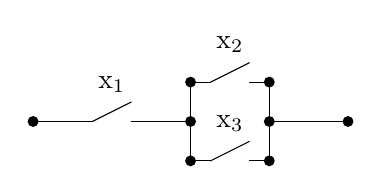
\begin{tikzpicture}
[circuit ee IEC]
\node [contact] (mid1) at (0, 0.5) {};
\node [contact] (mid4) at (4, 0.5) {};
\foreach \i in {2,...,3}{
	\node [contact] (up\i) at (\i, 1) {};
	\node [contact] (mid\i) at (\i, 0.5) {};
	\node [contact] (down\i) at (\i, 0) {};
}
\draw (mid1) to [make contact = {midway, info = x$_1$}] (mid2);
\draw (mid2) to (up2);
\draw (mid2) to (down2);

\draw (up2) to [make contact = {midway, info = x$_2$}] (up3);
\draw (down2) to [make contact = {midway, info = x$_3$}] (down3);

\draw (up3) to (mid3);
\draw (down3) to (mid3);
\draw (mid3) to (mid4);
\end{tikzpicture}

\end{document}
